\documentclass{beamer}

\mode<presentation>
{
  \usetheme{Frankfurt}
  \usecolortheme{orchid}
  \setbeamercovered{invisible}
  \setbeamertemplate{footline}[frame number]
}

\usepackage[english]{babel}
\usepackage[latin1]{inputenc}
\usepackage{times}
\usepackage[T1]{fontenc}
\usepackage{tikz}
\usepackage{array}
\usepackage{cancel}


\usetikzlibrary{shapes,backgrounds}

\def\multiset#1#2{\ensuremath{\left(\kern-.3em\left(\genfrac{}{}{0pt}{}{#1}{#2}\right)\kern-.3em\right)}}

\def\blue{\color{blue}~}
\def\black{\color{black}~}
\def\bl[#1]#2{\begin{block}{#1}#2\end{block}}
\def\integers{\mathbb{Z}}
\def\enumb{\begin{enumerate}}
\def\enume{\end{enumerate}}
\def\itemb{\begin{itemize}}
\def\iteme{\end{itemize}}


\usepackage{remreset}
\makeatletter
\@removefromreset{subsection}{section}
\makeatother
\setcounter{subsection}{1}

\title{Discrete Mathematics, Section 002, Spring 2016}
\subtitle{Lecture 11: Induction}

\author[Zsolt]{Zsolt Pajor-Gyulai \\ \texttt{zsolt@cims.nyu.edu}}

\pgfdeclareimage[height=1cm]{NYUlogo}{NYUlogo.jpg}

\institute[NYU] 
{
\normalsize Courant Institute of Mathematical Sciences
}
\titlegraphic{\pgfuseimage{NYUlogo}}

\begin{document}

\begin{frame}
  \titlepage
\end{frame}

\AtBeginSection[]
{
\begin{frame}
\frametitle{Outline}
\tableofcontents[currentsection]
\end{frame}}

\section{Induction}

\begin{frame}{The induction machine}
\begin{columns}
\column{0.55\textwidth}
What does it take for a line of Dominos to fall?
\enumb
\item We need to be able to tip over the first domino.
\item We need to be sure that whenever a domino falls, it knocks over the next Domino in the line.
\enume
If these two things are satisfied, we can be sure that all the Domino's will fall.
\column{0.45\textwidth}
\begin{figure}
\centering
\includegraphics[scale=0.1]{dominos}
\end{figure}
\end{columns}
\end{frame}

\begin{frame}{The induction machine}
\bl[Proposition]{Let $n$ be a positive integer. The sum of the first $n$ odd natural numbers is $n^2$.}
This is a statement about infinitely many equations:
\begin{align*}
1&=1^2\\
1+3&=2^2\\
1+3+5&=3^2\\
1+3+5+7&=4^2\\
&\vdots
\end{align*}
We could ask a computer to check each equation but it would last forever.
\end{frame}

\begin{frame}{The induction machine}
\bl[Proposition]{Let $n$ be a positive integer. The sum of the first $n$ odd natural numbers is $n^2$.}
\center We are going to build a different kind of machine:
\begin{figure}
\flushleft
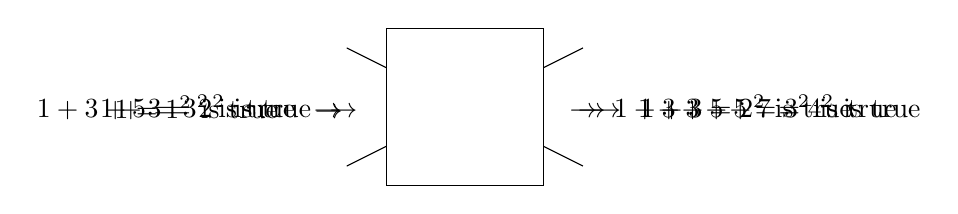
\begin{tikzpicture}[scale=0.5]
\draw (0,0) rectangle (4,4);
\draw (-1,3.5) -- (0,3);
\draw (-1,0.5) -- (0,1);
\draw (4,3) -- (5,3.5);
\draw (4,1) -- (5,0.5);

\uncover<2-3>{
\node at (-4,2) {$1=1^2$ is true $\quad\rightarrow$}; 
}
\uncover<3>{
\node at (8,2) {$\quad\rightarrow\quad 1+3=2^2$ is true};
}

\uncover<4-5>{
\node at (-4,2) {$1+3=2^2$ is true $~\rightarrow$}; 
}
\uncover<5>{
\node at (9,2) {$~\rightarrow~ 1+3+5=3^2$ is true};
}

\uncover<6-7>{
\node at (-5,2) {$1+3+5=3^2$ is true $~\rightarrow$}; 
}
\uncover<7>{
\node at (9,2) {$~\rightarrow~ 1+3+5+7=4^2$ is true};
}
\end{tikzpicture}
\end{figure}
\end{frame}

\begin{frame}{The induction machine}
\bl[Proposition]{Let $n$ be a positive integer. The sum of the first $n$ odd natural numbers is $n^2$.}
If we can make sure that the machine works a $100\%$ reliably, then we could just loop the output back on the input and `ignite it with the first equation'.
\begin{figure}
\centering
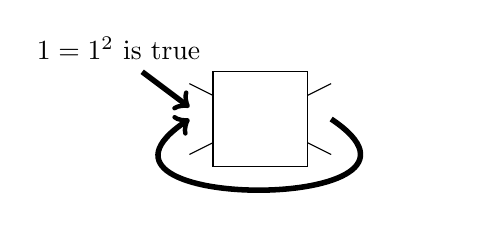
\begin{tikzpicture}[scale=0.3]
\draw (0,0) rectangle (4,4);
\draw (-1,3.5) -- (0,3);
\draw (-1,0.5) -- (0,1);
\draw (4,3) -- (5,3.5);
\draw (4,1) -- (5,0.5);

\draw[line width=2pt,->] (5,2) .. controls (11,-2) and (-7,-2) .. (-1,2);
\draw[line width=2pt,->] (-3,4) -- (-1,2.5);
\node at (-4,5) {$1=1^2$ is true};
\end{tikzpicture}
\end{figure}
Then we can be sure, all the equations will be proved eventually, just as we could be sure that all the dominos will fall.
\end{frame}

\begin{frame}{The induction machine}
\bl[Proposition]{Let $n$ be a positive integer. The sum of the first $n$ odd natural numbers is $n^2$.}
\enumb
\item Can we ignite? \uncover<2>{$\rightarrow$ Yes.}
\[
\textrm{Obviously } 1=1^2.
\]
\item Is the machine flawless? \uncover<2>{$\rightarrow$ Yes.}
\[
\textrm{Feed: $1+3+5+\dots+(2k-1)=k^2$ is true}
\]
Assuming this, add $2k+1$ to both sides and get
\begin{align*}
1+3+\dots+(2k-1)+(2k+1)&=k^2+(2k+1)=\\
&=k^2+2k+1=(k+1)^2.
\end{align*}\vspace{-0.8cm}

Therefore the output is\vspace{-0.3cm}

\[
1+3+5+\dots(2k+1)=(k+1)^2\textrm{ is true}.
\]
\enume
\end{frame}

\begin{frame}{Principle of mathematical induction}
\bl[Theorem]{Let $A$ be a set of natural numbers. If 
\itemb
\item $0\in A$, and
\item $\forall k\in\mathbb{N}: ( k\in A\Rightarrow k+1\in A)$,
\iteme
then $A=\mathbb{N}$.}
\bl[Proof]{
Suppose for the sake of contradiction, that $A\neq\mathbb{N}$. Let $X=\mathbb{N}-A$, then $X\neq\emptyset$.\\
~~~~By the WOP, there is a smallest element in $X$. Note that $x\neq 0$ because $0\in A$ is given. Therefore $x-1\in A$ by the definition of $x$. \\
~~~~By the second assumption, $x=(x-1)+1\in A$, which is a contradiction.$\Rightarrow\Leftarrow$
}
\end{frame}

\begin{frame}{Principle of mathematical induction}
\bl[Proof by induction]{
To prove that every natural number has some property:\\
\itemb
\item Let $A$ be the subset of $\mathbb{N}$ for which the result is true.
\item (Basis step) Prove that $0\in A$.
\item (Inductive step) Prove that if $k\in A$, then $k+1\in A$. To do this:
\itemb
\item Assume that the result is true for $n=k$. (Induction hypothesis)
\item Use the induction hypothersis to prove the result for $n=k+1$.
\iteme
\item By the POMI, conclude $A=\mathbb{N}$.
\iteme
Therefore the result is true for all natural numbers.
}
\end{frame}

\begin{frame}{An example}
\bl[Proposition]{Let $n\in\mathbb{N}$. Then
\[
0^2+1^2+\dots n^2=\frac{(2n+1)(n+1)n}{6},\qquad (*)
\]}

\bl[Proof]{
We prove this result by induction on $n$. Let $A\subseteq\mathbb{N}$ be the subset for which the claim is true.
\itemb
\item \textbf{Basis step:} Note that when $n=0$, both sides of $(*)$ is zero and therefore $n\in A$.
\item \textbf{Induction hypothesis:} Suppose the result is true for $n=k$, i.e. $k\in A$ and \vspace{-0.3cm}
\[
0^2+1^2+\dots+k^2=\frac{(2k+1)(k+1)k}{6},\qquad (**).
\]
\iteme\vspace{-0.5cm}
[...]
}
\end{frame}

\begin{frame}
\bl[Proposition]{Let $n\in\mathbb{N}$. Then\vspace{-0.3cm}
\[
0^2+1^2+\dots n^2=\frac{(2n+1)(n+1)n}{6},\qquad (*)
\]}

\bl[Proof]{
[...]\vspace{-0.2cm}
\itemb
\item \textbf{Induction step:} Now we show that under the induction hypothesis, the result holds for $n=k+1$. Indeed, add $(k+1)^2$ to both sides of $(**)$,
\begin{align*}
0^2+1^2+\dots (k+1)^2&=\frac{(2k+1)(k+1)k}{6}+(k+1)^2=\\
(\textrm{Probl 1 on WS})&=\frac{[(2(k+1)+1][(k+1)+1][k+1]}{6}.
\end{align*}
and therefore $k+1\in A$.
\iteme
[...]}
\end{frame}

\begin{frame}{An example}
\bl[Proposition]{Let $n\in\mathbb{N}$. Then
\[
0^2+1^2+\dots n^2=\frac{(2n+1)(n+1)n}{6},\qquad (*)
\]}
\begin{proof}

[...]
\itemb
\item We have shown that $0\in A$ and $(k\in A)\Rightarrow [(k+1)\in A]$. Therefore, by induction, $A=\mathbb{N}$ and the claim is true for all natural numbers.
\iteme
\end{proof}
\end{frame}

\begin{frame}{The basis step doesn't need to be about $0$.}

\bl[Proposition]{Let $n$ be a positive integer. Then
\[
2^0+2^1+\dots+2^{n-1}=2^n-1
\]}

\bl[Proof]{
We prove this by induction on $n$.\\\
~~~~ \textbf{Basis step:} The case $n=1$ is true because $2^0=1$ and $2^{1}-1$.\\
~~~~ \textbf{Induction hypothesis:} Suppose the result is true for $n=k$, i.e.
\[
2^0+2^1+\dots+2^{k-1}=2^k-1,\qquad (***)
\]
[...]
}
\end{frame}

\begin{frame}{The basis step doesn't need to be about $0$.}

\bl[Proposition]{Let $n$ be a positive integer. Then
\[
2^0+2^1+\dots+2^{n-1}=2^n-1.
\]}

\bl[Proof]{
[...]\\
~~~~\textbf{Induction step:} Now we show that under the ind. hyp., the result is true for $n=k+1$. Indeed by adding $2^k$ to both sides of $(***)$,
\[
2^0+2^1+\dots+2^{k}=2^k+1+2^k=2\cdot 2^{k}+1=2^{k+1}+1.
\]
which is exatly what we needed to show.
}
\center Practice this on Problem 2, (a)-(c) on the worksheet!
\end{frame}

\begin{frame}{Example with an inequality}
\bl[Proposition]{Let $n$ be a natural number. Then\vspace{-0.3cm}
\[
10^0+10^1+\dots+10^n<10^{n+1}
\]}
\begin{proof}
The proof is by induction on $n$. The basis case, when $n=0$, is clear because $10^0<10^1$.

~~~~ Assume that the result holds for $n=k$; that is, we have\vspace{-0.3cm}
\[
10^0+10^1+\dots+10^k<10^{k+1}.\vspace{-0.3cm}
\]

To show that the Proposition is true when $n=k+1$, we add $10^{k+1}$ to both sides and find\vspace{-0.3cm}
\begin{align*}
10^0+&10^1+\dots 10^{k+1}<10^{k+1}+10^{k+1}=\\
&=2\cdot 10^{k+1}<10\cdot 10^{k+1}=10^{k+2}.
\end{align*}\vspace{-0.7cm}

Therefore the result holds when $n=k+1$.\qedhere
\end{proof}
\end{frame}

\begin{frame}
\center Now do Problem 2 (d)-(e).
\end{frame}

\begin{frame}{Further example}
\bl[Proposition]{Let $n\in\mathbb{N}$. Then $4^n-1$ is divisible by $3$.}

\begin{proof}
The proof is by induction on $n$. The basis case, $n=0$, is clear since $4^0-1=1-1=0$ is divisible by $3$.

~~~~ Suppose that the result is true for $n=k$; that is, $3|4^k-1$. To show that then the result is also true for $n=k+1$, note
\[
4^{k+1}-1=4\cdot 4^k-1=4(4^k-1)+4-1=4(4^k-1)+3.
\]
Since $4^k-1$ and $3$ are both divisible by $3$, it follows that $4(4^k-1)+3$ is also divisible by $3$, which means that $4^{k+1}-1$ is divisible by $3$ too.
\end{proof}

\end{frame}

\section{Strong Induction}

\begin{frame}{Principle of Mathematical Induction - strong version}
We like induction, because
\itemb
\item The basis case is usually easy.
\item When proving the induction step we can work with the case $n=k$ assumed true by the induction hypothesis.
\item This means that we have a lot more to work with than just the assumptions of the theorem.
\iteme

On the other hand note that we have something even more.
\itemb
\item When the machine proves $k\to k+1$, it has already proved
\[
0\to 1\to 2\to\dots\to k-1\to k.
\]
\item This means that we can proceed cumulatively, i.e.
\[
0\to 1,\qquad 0,1\to 2\qquad 0,1,2\to 3\qquad\dots\qquad
\]
\[
\dots\qquad 0,1,\dots,k\to k+1.
\]
\iteme
\end{frame}

\begin{frame}{Principle of Mathematical Induction - strong version}
\bl[Theorem]{
Let $A$ be a set of natural numbers. If
\itemb
\item $0\in A$ and
\item for all $k\in\mathbb{N}$, $0,1,\dots,k\in A$ implies $k+1\in A$,
\iteme
then $A=\mathbb{N}$.}

\bl[]{
To prove that every natural number has some property:
\itemb
\item Let $A$ be the set of natural numbers for which the result is true.
\item Prove $0\in A$. (Basis step)
\item Prove that $0,1,\dots, k\in A$ implies $k+1\in A$. (inductive step)
\item By the SPOMI, $A=\mathbb{N}$.
\iteme}
\end{frame}

\begin{frame}{An example}
\bl[Definition]{A \textbf{triangulation} of a polygon is to draw diagonals through the interior of the poligons so that
\itemb
\item The diagonals do not cross each other.
\item Every region created is a triangle.
\iteme}
\begin{figure}
\centering
\begin{tikzpicture}[scale=0.8]
\draw[line width = 2pt] (0,1) -- (2,3) -- (5,2)  -- (6,0) -- (4,-1) -- (1.5,-0.5) -- (0,1);

\only<1>{\draw [blue] (0,1) -- (5,2) -- (1.5,-0.5) -- (6,0);}
\only<2>{\draw [blue] (2,3) -- (1.5,-0.5); \draw[blue] (2,3) -- (4,-1) -- (5,2);}
\end{tikzpicture}
\end{figure}
\end{frame}

\begin{frame}{An example}
\bl[Definition]{A triangle in a triangulation is \textbf{exterior} if two of their three sides are on the exterior of the original polygon.}
\begin{figure}
\centering
\begin{tikzpicture}[scale=0.8]
\draw[line width = 2pt] (0,1) -- (2,3) -- (5,2)  -- (6,0) -- (4,-1) -- (1.5,-0.5) -- (0,1);

\only<1>{\draw [blue] (0,1) -- (5,2) -- (1.5,-0.5) -- (6,0);
\fill[blue] (0,1) -- (2,3) -- (5,2) -- (0,1);
\fill[blue] (6,0) -- (4,-1) -- (1.5,-0.5) -- (6,0);}

\only<2>{\draw [blue] (2,3) -- (1.5,-0.5); \draw[blue] (2,3) -- (4,-1) -- (5,2);
\fill[blue] (0,1) -- (2,3) -- (1.5,-0.5) -- (0,1);
\fill[blue] (6,0) -- (4,-1) -- (5,2) -- (6,0);}

\end{tikzpicture}
\end{figure}
\end{frame}

\begin{frame}
\bl[Proposition]{If a polygon with four or more sides is triangulated, then at least two of the triangles formed are exterior.}

\bl[Proof]{
Let $n$ be the number of sides of the polygon. We prove the Proposition by strong induction on $n$.\\
~~~\textbf{Base case:} For $n=4$, the only way to triangulate the polygon is to draw in one of the two possible diagonals. Each way, the resulting two triangles are exterior.
\begin{figure}
\begin{tikzpicture}[scale=0.8]
\draw[line width=2pt] (0,0) -- (1,2) -- (3,3) -- (4,1) -- (0,0);
\only<2>{\draw[blue] (0,0) -- (3,3);}
\only<3>{\draw[blue] (1,2) -- (4,1);}
\end{tikzpicture}
\end{figure}\vspace{-0.5cm}
[...]
}
\end{frame}

\begin{frame}
\bl[Proposition]{If a polygon with four or more sides is triangulated, then at least two of the triangles formed are exterior.}

\bl[Proof]{
[...]\\
~~~\textbf{Strong induction hypothesis:} Suppose that the result has been proved for all polygons with $n=4,5,...,k$ sides and let $P$ be any triangulated polygon with $k+1$ sides. We will show that at least two of the sides are exterior.
\begin{columns}
\column{0.45\textwidth}
\begin{figure}
\flushright
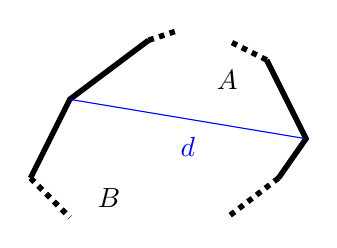
\begin{tikzpicture}[scale=0.5]
\draw[line width=2pt] (0,0) -- (1,2) -- (3,3.5);
\draw[line width =2pt] (6,3) -- (7,1) -- (6.3,0);
\draw[blue] (1,2) -- (7,1);
\draw[line width=2pt, dotted] (3,3.5) -- (3.75,3.75);
\draw[line width=2pt, dotted] (6,3) -- (5,3.5);
\draw[line width=2pt, dotted] (0,0) -- (1,-1);
\draw[line width=2pt, dotted] (6.3,0) -- (5,-1);
\node[blue] at (4,0.8) {$d$};
\node at (5,2.5) {$A$};
\node at (2,-0.5) {$B$};
\end{tikzpicture}
\end{figure}
\column{0.55\textwidth}
Let $d$ be one of the diagonals. Then $d$ separates $P$ into two triangulated polygons $A$ and $B$\\ with fewer sides than $P$.
\end{columns}
[...]
}
\end{frame}

\begin{frame}
\bl[Proposition]{If a polygon with four or more sides is triangulated, then at least two of the triangles formed are exterior.}

\bl[Proof]{
[...]\vspace{-0.2cm}
\itemb
\item If $A$ is not a triangle, then since $A$ has at least four but at most $k$ sides, the strong induction hypothesis implies that two or more $A$-triangles are exterior to $A$. The only way for one of these triangles not to be exterior to $P$ as well is if one of the sides is $d$. Since that can happen to at most one of the triangles exterior to $A$, the other one also has to be exterior to $P$.
\item If $A$ is a triangle then $A$ is an exterior triangle.
\item Similarly, there is a triangle in $B$ exterior to $P$.
\iteme
Therefore, we have at least two exterior triangles to $P$.\qed
}
\end{frame}

\begin{frame}
\center{Do problem 3-4 on the worksheet!}
\end{frame}




\end{document}